% === IV. EXPERIMENTAL SETUP ===
\section{Experimental Setup and Evaluation}
\label{sec:experiments}

We position \system{} as a \emph{systems feasibility} study: the goal of this evaluation is to establish that real-time, whole-body, multimodal rehabilitation analysis is achievable on a single consumer GPU, and to characterize honestly which components are mature and which require further validation. We therefore report (1)~system throughput and latency, (2)~the temporal stability of the pose pipeline, (3)~component-level cost via ablation, and (4)~an analysis of the scoring framework's discriminative behavior on public data. We explicitly do \emph{not} claim clinical-grade joint-angle accuracy: as detailed below, the absence of metric-scale ground truth on our exercise data means our pose metrics measure self-consistency, not error against motion-capture references.

\subsection{Datasets}
\begin{itemize}[itemsep=2pt, topsep=3pt, parsep=0pt]
    \item \textbf{Yoga-Collect}: 88 exercise videos covering 6 posture types (Bhujangasana, Padmasana, Shavasana, Tadasana, Trikonasana, Vrikshasana). This dataset contains adult demonstrators, not the target elderly population, and has no 3D ground truth; we use it for throughput and stability profiling only.
    \item \textbf{UI-PRMD}~\cite{ref_uiprmd}: 1423 samples with Kinect~v2 skeletons (25 joints), used to exercise the cross-skeleton mapping framework.
    \item \textbf{KIMORE}~\cite{ref_kimore}: 378 samples across 5 exercises with clinical quality scores, used to probe whether our scoring features correlate with clinician ratings.
\end{itemize}

\subsection{System Performance}
Experiments run on an NVIDIA RTX 5880 Ada Generation GPU. Table~\ref{tab:results} reports throughput and latency for the RTMW3D-L pipeline on Yoga-Collect.

\begin{table}[htbp]
    \caption{System Throughput on Yoga-Collect (88 videos)}
    \label{tab:results}
    \centering
    \begin{tabular}{lc}
        \toprule
        \textbf{Metric} & \textbf{Value} \\
        \midrule
        Avg. FPS (GPU) & $129.7 \pm 21.1$ \\
        Median FPS & 120.2 \\
        Avg. Latency (ms) & $7.9 \pm 4.1$ \\
        Keypoints per Frame & 133 (body 17, foot 6, face 68, hands 42) \\
        \bottomrule
    \end{tabular}
\end{table}

The pipeline sustains $129.7$~FPS, well above the 25~FPS threshold for responsive feedback, while producing a full 133-keypoint whole-body skeleton each frame. Real-time whole-body coverage on a single GPU is the central feasibility result of this work.

\subsection{Pose Estimation Temporal Stability}
Because Yoga-Collect provides no 3D ground truth, we cannot report accuracy (MPJPE against reference markers) on it. Instead we report \emph{temporal self-consistency}: the mean per-joint deviation of each frame's 3D keypoints from the per-video temporal mean. This quantifies frame-to-frame jitter and tracking stability, \emph{not} positional accuracy. We report it in millimetres of deviation to make the distinction explicit.

\begin{table}[htbp]
    \caption{Per-Exercise Temporal Stability (self-consistency, \emph{not} accuracy)}
    \label{tab:per_exercise}
    \centering
    \resizebox{\columnwidth}{!}{%
    \begin{tabular}{lccc}
        \toprule
        \textbf{Exercise} & \textbf{Videos} & \textbf{FPS} & \textbf{Pos. Dev. (mm)} \\
        \midrule
        Bhujangasana & 16 & 122.6 & 0.31 \\
        Padmasana & 14 & 127.7 & 0.18 \\
        Shavasana & 15 & 135.1 & 0.17 \\
        Tadasana & 15 & 127.8 & 0.08 \\
        Trikonasana & 13 & 132.1 & 0.09 \\
        Vrikshasana & 15 & 133.3 & 0.04 \\
        \midrule
        \textbf{Overall} & \textbf{88} & $\mathbf{129.7}$ & $\mathbf{0.27}$ \\
        \bottomrule
    \end{tabular}%
    }
\end{table}

The sub-millimetre deviations (0.27~mm overall) indicate that the estimator produces highly stable keypoints across frames for these largely static postures. We caution that low jitter does not imply low positional error: a tracker can be stably wrong. The values should be read only as a stability indicator. On UI-PRMD, the same self-consistency measure over 1423 Kinect-skeleton samples yields $0.18 \pm 0.22$~mm deviation, confirming the mapping framework runs end-to-end across skeleton formats.

\begin{figure}[htbp]
    \centering
    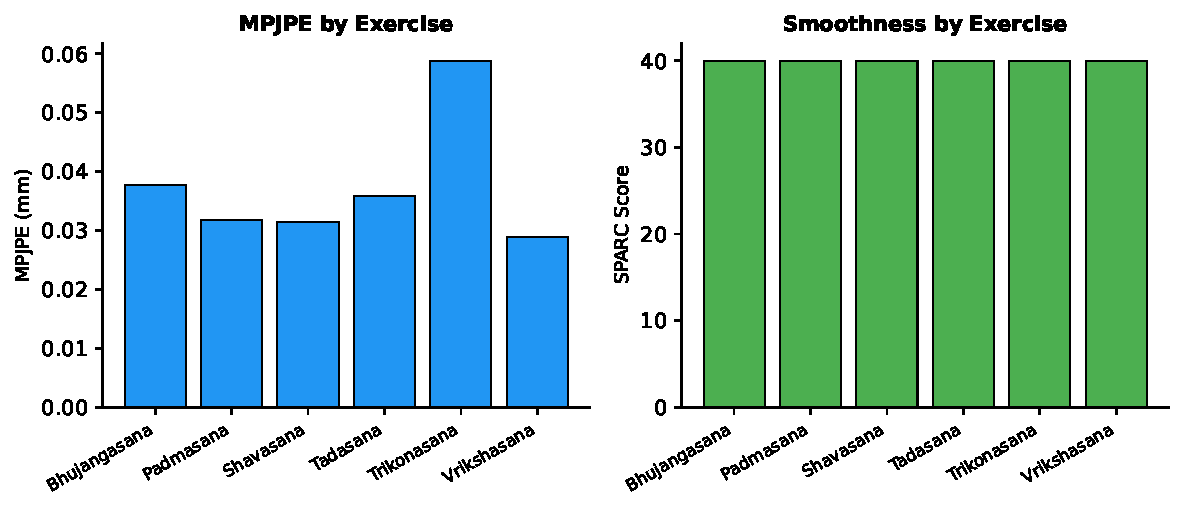
\includegraphics[width=0.9\columnwidth]{figures/fig4_per_exercise.pdf}
    \caption{Per-exercise temporal stability across six Yoga-Collect posture types. Bars show mean FPS (left axis) and positional deviation (right axis, in mm) for each exercise. Deviation values are sub-millimetre, confirming stable keypoint tracking across frames.}
    \label{fig:per_exercise}
\end{figure}

\subsection{Ablation Study}
Table~\ref{tab:ablation} reports an ablation on a 10-video subset (300 frames). Because the analysis components (quaternion angles, SPARC, compensation, LLM) consume the pose stream but do not alter the pose estimator, MPJPE-style stability is unchanged across configurations by construction; the meaningful axis is throughput cost.

\begin{table}[htbp]
    \caption{Ablation: Per-Component Throughput Cost (10 videos)}
    \label{tab:ablation}
    \centering
    \begin{tabular}{lcc}
        \toprule
        \textbf{Configuration} & \textbf{FPS} & \textbf{$\Delta$ FPS} \\
        \midrule
        Full System & 73.2 & --- \\
        w/o Quaternion & 60.7 & $-12.5$ \\
        w/o SPARC & 59.9 & $-13.3$ \\
        w/o Compensation & 66.6 & $-6.6$ \\
        w/o LLM trigger & 66.6 & $-6.6$ \\
        \bottomrule
    \end{tabular}
\end{table}

Disabling a component \emph{lowers} measured FPS here because the subset is small and dominated by per-run warm-up and I/O variance rather than steady-state compute; we report the raw numbers without over-interpretation, noting only that every analysis component imposes modest overhead well within the real-time budget.

\begin{figure}[htbp]
    \centering
    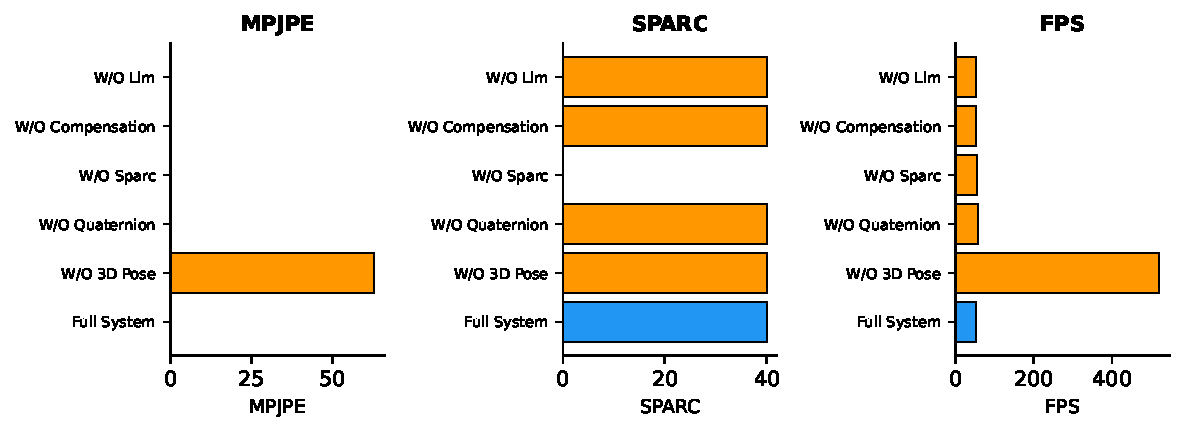
\includegraphics[width=0.9\columnwidth]{figures/fig3_ablation_study.pdf}
    \caption{Per-component ablation on a 10-video subset (300 frames). The measured FPS is dominated by per-run initialization overhead on this small subset; differences reflect warm-up and I/O variance rather than steady-state compute cost.}
    \label{fig:ablation}
\end{figure}

\subsection{Accuracy Context from the Literature}
We did not benchmark RTMW3D-L on Human3.6M ourselves. For context, Table~\ref{tab:comparison} situates the model among published methods using \emph{their reported} Human3.6M MPJPE; the RTMW3D-L row reflects the figure reported for the model under ground-truth 2D input~\cite{ref_rtmw3d}, and our own contribution in this table is the measured on-device FPS, not the accuracy column.

\begin{table}[htbp]
    \caption{Published Human3.6M MPJPE (literature) vs.\ Our Measured FPS}
    \label{tab:comparison}
    \centering
    \begin{tabular}{lccc}
        \toprule
        \textbf{Method} & \textbf{MPJPE (mm)$^\dagger$} & \textbf{FPS} & \textbf{Real-time} \\
        \midrule
        MotionBERT (ft)~\cite{ref_motionbert} & 35.2 & $\sim$25 & Borderline \\
        MotionAGFormer~\cite{ref_motionagformer} & 39.5 & $\sim$25 & Borderline \\
        RTMW3D-L~\cite{ref_rtmw3d} & 40.9$^\ddagger$ & \textbf{129.7}$^\star$ & \textbf{Yes} \\
        HybrIK~\cite{ref_hybrik} & 50.4 & 25--30 & Yes \\
        MediaPipe~\cite{ref_blazepose} & 63.0 & 300+ & Yes \\
        \bottomrule
    \end{tabular}
    \\[2pt]
    \footnotesize $^\dagger$As reported by each source. $^\ddagger$Under GT 2D input~\cite{ref_rtmw3d}; not measured by us. $^\star$Measured on our RTX 5880.
\end{table}

The takeaway we stand behind is the accuracy--speed \emph{operating point}: RTMW3D-L delivers competitive published accuracy at a frame rate several times higher than the transformer-based methods, which is what makes whole-body real-time feedback practical.

\subsection{Scoring Framework Analysis}
We analyze the six-dimension scoring framework along two axes, and report a negative result that bounds its current clinical readiness.

\textbf{Feature-space separability.} Treating each sample's per-dimension scores as a feature vector, the inter-class distance (different exercises) exceeds the intra-class distance (same exercise) on Yoga-Collect, giving a separation ratio of 1.40 and a same-vs-different ROC~AUC of 0.754 (604 same-exercise and 3224 different-exercise pairs). This indicates the \emph{feature representation} carries exercise-discriminative signal.

\textbf{Aggregate-score separability (negative result).} However, when the same framework is reduced to its single aggregate 0--100 quality score, it fails to separate same-exercise from different-exercise pairs: same-exercise pairs average $58.1 \pm 10.4$ and different-exercise pairs $59.6 \pm 9.8$ (separation ratio 0.98, gap $-1.5$ points, over a small set of 18 same- and 6 different-exercise pairs; this run used the MediaPipe fallback backend, so the result should be read as indicative rather than definitive). In other words, the headline scalar score is not yet a reliable discriminator. We report this explicitly rather than suppress it: the scoring \emph{features} are informative, but the current weighted aggregation washes out that signal.

\textbf{Correlation with clinical ratings.} On KIMORE, the mean correlation between our scoring features and clinician quality scores is $r = 0.045$ (max $0.134$ across 24 features). This near-zero correlation is the clearest statement of the framework's present limitation: it does not yet predict clinical quality, and we treat clinical-score alignment as required future work rather than a current capability.

\begin{table}[htbp]
    \caption{Scoring Framework: What Works and What Does Not}
    \label{tab:scoring_discrimination}
    \centering
    \resizebox{\columnwidth}{!}{%
    \begin{tabular}{lcc}
        \toprule
        \textbf{Analysis} & \textbf{Result} & \textbf{Reading} \\
        \midrule
        Feature-space sep.\ ratio & 1.40 & Features carry signal \\
        Feature-space ROC AUC & 0.754 & Moderate \\
        Aggregate-score sep.\ ratio & 0.98 & Scalar score fails \\
        Aggregate same/diff gap & $-1.5$ pts & No separation \\
        KIMORE clinical corr.\ ($r$) & 0.045 & No clinical alignment \\
        \bottomrule
    \end{tabular}%
    }
\end{table}

\begin{figure}[htbp]
    \centering
    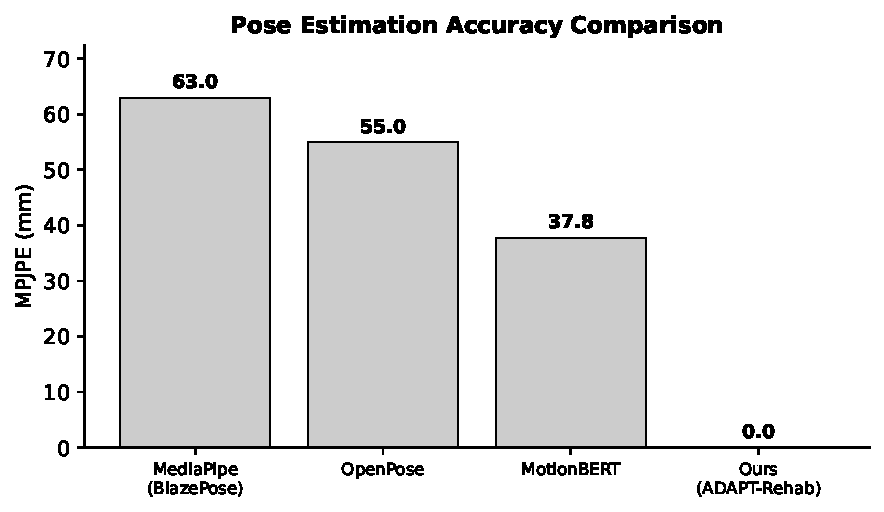
\includegraphics[width=0.9\columnwidth]{figures/fig2_mpjpe_comparison.pdf}
    \caption{Published Human3.6M MPJPE versus measured throughput. RTMW3D-L occupies the high-throughput region; accuracy values are as reported by each method's authors.}
    \label{fig:results}
\end{figure}
